\documentclass[english,11pt]{article}
\usepackage[T1]{fontenc}
\usepackage[latin9]{inputenc}
\usepackage{geometry}
\usepackage{graphicx}
\usepackage{float}
\usepackage{subcaption} % to plot subfigure
\usepackage[linesnumbered,ruled,vlined]{algorithm2e}
\geometry{verbose,tmargin=2.5cm,bmargin=2.5cm,lmargin=2.5cm,rmargin=2.5cm}
\usepackage{amsmath}
\usepackage{babel}
\begin{document}







%%%%%%%%%%%%%%%%%%%%%%%%%%%%%%%%%%%%
%%%%%%%%%% part 0 %%%%%%%%%%%%%%%%%%
%%%%%%%%%%%%%%%%%%%%%%%%%%%%%%%%%%%%
\part*{Bonus question:}
\subsection*{ 4.1 Regularized Linear Regression}
Figure~\ref{fig:4_1}  plots the variation in training/testing error with $\lambda$ for regularized linear model.
\begin{itemize}
\item Best $\lambda=10$:
\item training error: 11.605155
\item test error: 12.6566689644
\end{itemize}

\begin{figure}[ht]
\centering
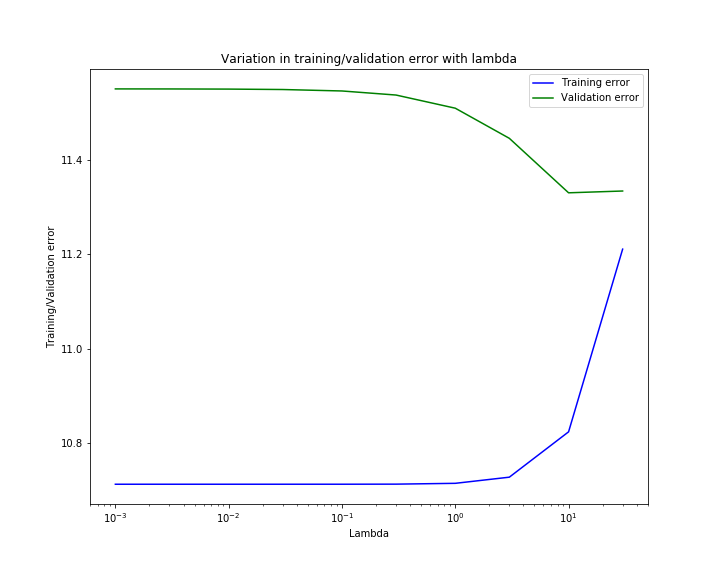
\includegraphics[width=.5\textwidth]{../hw1/part2/fig4_linear_lambda_10.png}
\caption{Variation in training/testing error with $\lambda$ for regularized linear model}
\label{fig:4_1}
\end{figure}



\subsection*{ 4.2 Selecting $\lambda$ with quadratic features}
Figure~\ref{fig:4_2} plots the variation in training/testing error with $\lambda$ for regularized linear model with quadratic features.
\begin{itemize}
\item Best $\lambda=0.3$:
\item training error:  4.256794
\item test error: 4.82815820863
\end{itemize}

\begin{figure}[ht]
\centering
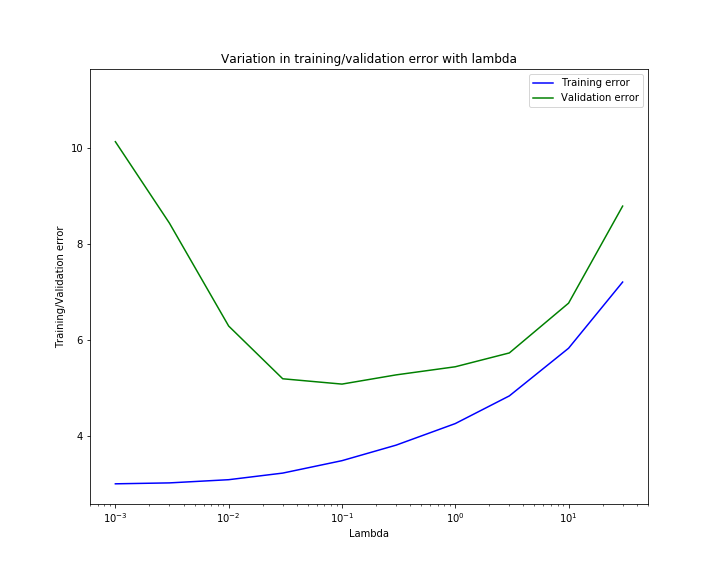
\includegraphics[width=.5\textwidth]{../hw1/part2/fig4_quadratic_lambda_03.png}
\caption{Variation in training/testing error with $\lambda$ for regularized linear model with quadratic features}
\label{fig:4_2}
\end{figure}




\subsection*{ 4.3 Selecting $\lambda$ with cubic features}
\begin{figure}[h]
\centering
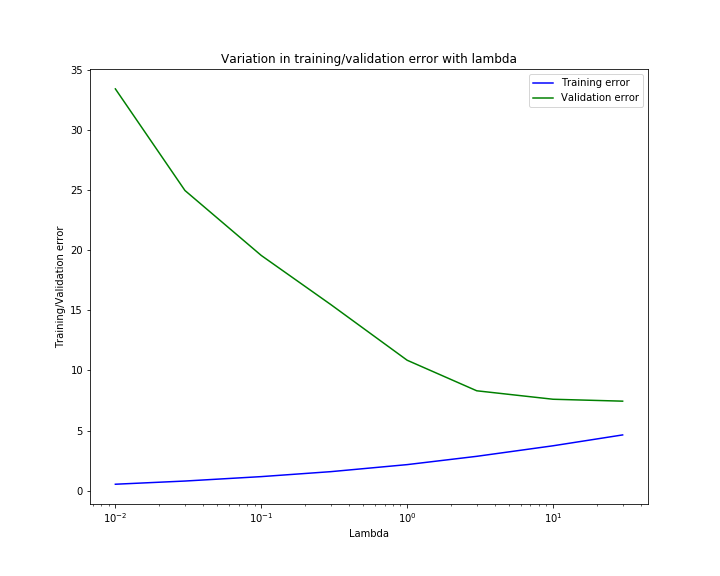
\includegraphics[width=.5\textwidth]{../hw1/part2/fig4_cubic_lambda_3.png}
\caption{Variation in training/testing error with $\lambda$ for regularized linear model with quadratic features}
\label{fig:4_3}
\end{figure}

Figure~\ref{fig:4_3} plots the variation in training/testing error with $\lambda$ for regularized linear model with quadratic features. 
\begin{itemize}
\item Best $\lambda=3$:
\item training error:  3.645624
\item test error: 4.73217608015
\end{itemize}







\subsection*{ Summary}
In above sections, we trained linear regression model with linear/quadratic/cubic features to predict Boston house price. We can observe that all three models we built embodied the power of regulation in that appropriate value of $\lambda$ gives the "sweet region" --- and even though the number of features grow dramatically as we square and even cube the features for more variation, the regulation term in the loss function successfully constrains the model from overfitting. The fact that models with linear, quadratic, cubic features are successively one better than the other shows that: given more features (variations) and proper control of overfitting, the more delicate model has better performance in prediction.




\end{document}
